%!TEX root = ../../main.tex
\chapter{Test and Verification}
As already mentioned in previous chapters, the whole EDRICO CPU is designed and implemented in many units. Since the approach using the V-model consists of working in bottom-up order for the implementation, test and verification processes, the first thing to implement and also test are the units of EDRICO. In the following chapters, the bottom-up way of the right side of the V-model (figure \ref{fig:vmod}) is described in detail.
\section{Unit Verification}
The first step in Test and Verification is the Unit Verification. In this step, the lowest units of the project are tested to prevent possible bugs from occurring in later stages of the verification. It is crucial to test every unit of the project because in a later stage of verification it is very complicated and time intensive to localize the bug and fix it in a top-down way. The main goal is to identify and fix bugs as early as possible. In this section, the unit verification process for the CU decoding unit is described in detail.\\
The task of the decoding unit is to parse the 32-bit instruction string, extract information and set the control signals respectively.\\
To get a better understanding of how the decoding process is executed, the source code of the decoder can be found in the appendix (\textbf{A. CU decoder}).\\
Unit verification starts by inserting source files of the implementation into a Xilinx Vivado\textcopyright  project. To test a unit, it is required to implement a so called testbench. This testbench will serve as a test environment for the \ac{UUT}. Testbenches are used for simulation purpose only (not for synthesis). Therefore, several VHDL constructs like \textit{assert}, \textit{report}, or \textit{loop} can be used. The corresponding testbench for the decoder can be found in the appendix (\textbf{B. CU decoder testbench}). During the testbench simulation, the UUT is stimulated with different input data. In this case, the decoder receives a different 32-bit instruction string. The following code shows how the stimulation process is implemented:
\begin{lstlisting}[style=vhdl, caption=CU testbench stimulation process]
stim: process
begin
	-- parse through different instruction strings
	--OPIMM
	ir <= "00000000001000100000000010010011"; --ADDI
	wait for 100ns;
	ir <= "00000000001000100010000010010011"; --SLTI
	wait for 100ns;
	ir <= "00000000001000100011000010010011"; --SLTIU
	wait for 100ns;
	ir <= "00000000001000100100000010010011"; --XORI
	...
\end{lstlisting}
To verify the functionality of the decoder unit, Vivado generates a timing diagram where it is possible to inspect all input and output signals of the UUT. The following figure \ref{fig:opimm} shows the timing diagram for the CU decoder testbench.
\begin{figure}[H]
	\centering
	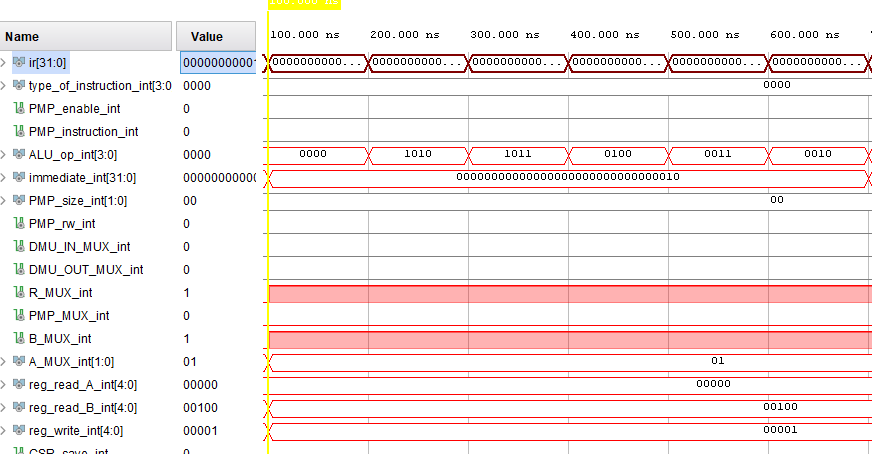
\includegraphics[width=\textwidth]{CUtbOPIMM}
	\caption{Vivado timing diagram for OPIMM instructions}
	\label{fig:opimm}
\end{figure}
For the OPIMM instruction cluster, the relevant output signals are highlighted in red. The top row shows how the instruction string is changing every 100 ns. As a result of that, the \textit{ALU\_op} signal changes, as the instruction changes. The first instruction is a \textit{ADDI} instruction which should lead to a 4-bit output signal of \textbf{0000}. After that a \textit{SLTI} instruction is inserted which should lead to a \textbf{1010} output (as shown in table \ref{aluop}). These outputs are correctly set as the timing diagram shows. The same validation technique is executed for all the other relevant signals. After establishing a correct signal for every output and every instruction, the unit can be declared as verified.\\
Figure \ref{fig:cutiming} shows the full timing diagram for the full testbench duration. It is visible that for example the memory signals are only active for memory operations.
\begin{figure}[H]
	\centering
	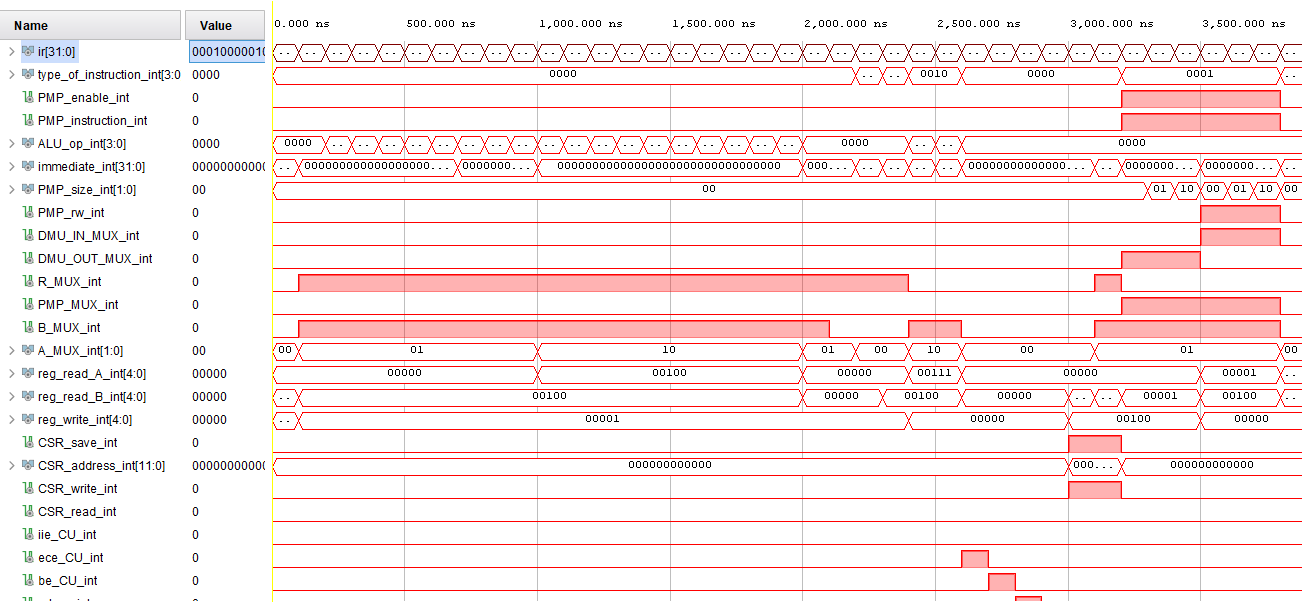
\includegraphics[width=\textwidth]{CUtiming}
	\caption{Vivado timing diagram for full CU decoder testbench}
	\label{fig:cutiming}
\end{figure}

Another unit that had to be verified outside of the control unit is the ALU. Since the complexity of the ALU is not as high as of the control unit, the testbench and also the timing diagram are very simple. The stimulation process of the ALU testbench is shown in the code below:
\begin{lstlisting}[style=vhdl, caption=CU testbench stimulation process]
stim: process
begin
	-- set input signal
	in_a <= "00000000000000000000000000000010";
	in_b <= "00000000000000000000000001000000";

	-- set op signal
	alu_op <= "0000"; --ADD
	wait for 100ns;
	alu_op <= "0001"; --SUB
	wait for 100ns;
	alu_op <= "0010"; --AND
	wait for 100ns;
	alu_op <= "0011"; --OR
	wait for 100ns;
	alu_op <= "0100"; --XOR
	wait for 100ns;
	alu_op <= "0101"; --EQUAL
	wait for 100ns;
	alu_op <= "0110"; --NEQUAL
	wait for 100ns;
	alu_op <= "0111"; --shift_left
	wait for 100ns; 
	alu_op <= "1000"; --shift_right
	wait for 100ns;
	alu_op <= "1001"; --shift_right (arithmetic)
	...
\end{lstlisting}
This code shows the first few operations that the ALU performs. First of all a pre defined input is fed to the ALU consisting of \textit{in\_a = 0x00000002} and \textit{in\_b = 0x00000040}. With these inputs, the different ALU operations are called using the \textit{alu\_op} signal. The following table \ref{table:alutb} will give an overview over what the expected results are:
\begin{table}[H]
	\setlength\arrayrulewidth{2pt}
	\centering
	\begin{tabular}{|c|c|c|}
		\hline
		\rowcolor{light-gray}
		\textbf{ALU\_OP} & \textbf{ALU\_result} & \textbf{branch\_re} \\
		\hline
		0000 (ADD) & 0x00000042 & 0 \\
		\hline
		0001 (SUB) & 0x0000003e & 0 \\
		\hline
		0010 (AND) & 0x00000000 & 0\\
		\hline
		0011 (OR) & 0x00000042 & 0\\
		\hline
		0100 (XOR) & 0x00000042 & 0\\
		\hline
		0101 (EQUAL)& 0x00000000 & 0\\
		\hline
		0110 (NEQUAL)& 0x00000000 & 1\\
		\hline
		0111 (shift\_left) & 0x00000100 & 0\\
		\hline
		1000 (shift\_right)& 0x00000010 & 0 \\
		\hline
		1001 (shift\_right (arith.))& 0x00000010 & 0\\
		\hline
	\end{tabular}
	\label{table:alutb}
	\caption{ALU testbench correct outputs}
\end{table}
The branch\_re output is only relevant for operations that can be called by branch instructions. In this case, the \textit{EQUAL} and \textit{NEQUAL} operations have to deliver a branch response. Apparently, the two inputs are not the same which is the reason for why the \textit{EQUAL} operation shall return 0 while the \textit{NEQUAL} operation shall return 1. The other operations are basic mathematical and arithmetical operations and the output is calculated by just performing the respective operations on the two inputs. After simulating the testbench in Vivado the resulting timing diagram (figure \ref{fig:alutb}) shows that everything works as desired. 
\begin{figure}[H]
	\centering
	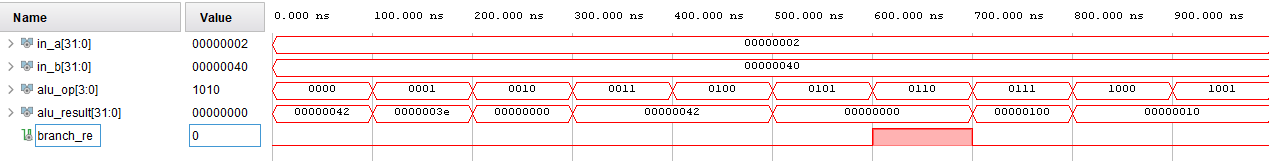
\includegraphics[width=\textwidth]{ALUtb}
	\caption{Vivado timing diagram for ALU testbench}
	\label{fig:alutb}
\end{figure}
With the same approach, every other unit is verified and occuring bugs are fixed until simulation and desired output are equal.
\section{Integration Verification}
During this stage of Test and Verification, all of the units have already been tested and verified. In this step, it is verified, that the units created and tested independently can coexist and communicate among themselves. In this project, the Integration Verification consists of creating so called \textit{top-files} which conclude all the corresponding units to a sub system. This section describes how the Control Unit of the EDRICO CPU went through this stage. 
\section{System Verification}